\chapter{Desenvolvimento da EDA}

Nesse capítulo, é aplicado os três passos do ciclo de uma EDA em um contexto prático aplicando o conjunto de dados "Brazilian Cities".

\section{Caso 1: Análise do IDH}

O IDH (Índice de Desenvolvimento Humano) é um índice que avalia a qualidade de vida em um determinado local, sendo mensurado a partir de 3 fatores: Longevidade, Educação e Renda. No Brasil, o órgão responsável por avaliar o IDH é o IBGE (Instituto Brasileiro de Geografia e Estatística).

Sendo um parâmetro importante, o IDH é capaz de influenciar tomadas de decisões, tais como quais setores aplicar investimento público pelos políticos, se é vantajoso mudar-se para morar nesse local, e se é viável a iniciativa privada investir nesse local para atuar.

Vide na figura \autoref{fig:distribuicao-idh-nas-cidades} a distribuição do IDH nas cidades do Brasil.

\begin{figure}[H]
  \centering
  \caption{\label{fig:distribuicao-idh-nas-cidades}Distribuição do IDH nas cidades brasileiras}
  \label{fig:der}
  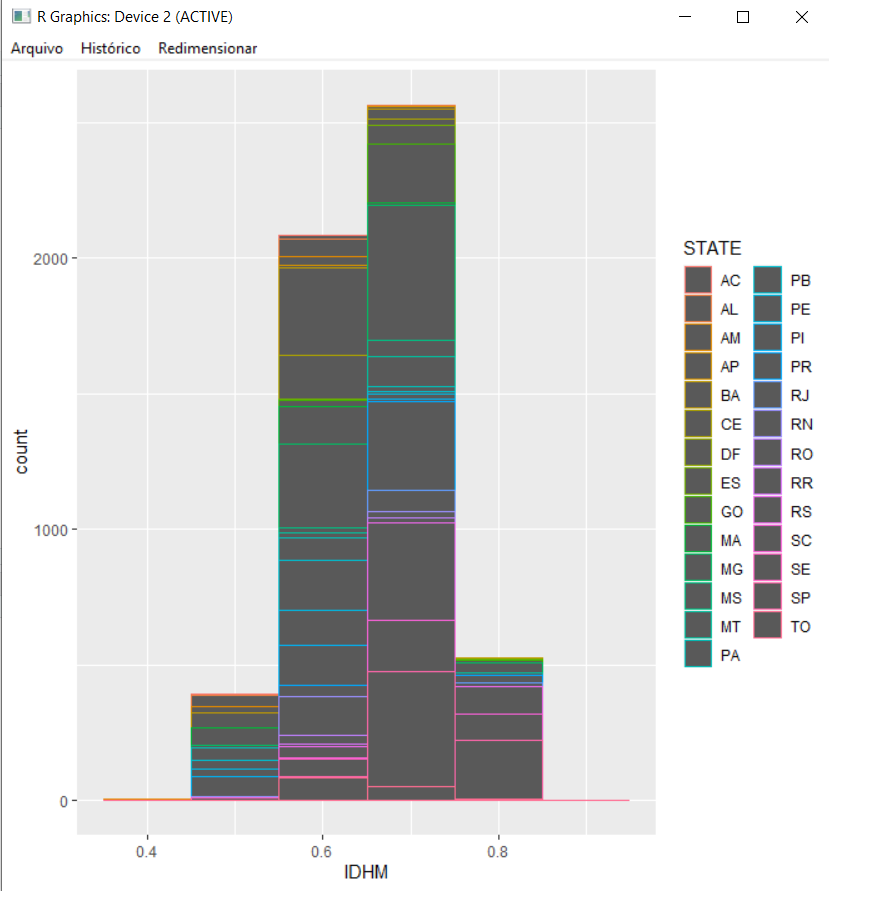
\includegraphics[scale=0.6]{chapter-03-case-01-img-01}
  \legend{Fonte: O autor}
\end{figure}

Visualizando esse gráfico, é perceber que não há cidades brasileiras com IDH menor do que 0.4, nem com IDH maior do que 0.8.

Com isso, surgem-se duas questões: 

\begin{enumerate}
	\item "Por que não existe IDH maior que 1?";
	\item "Q2?".
\end{enumerate}	

...

\section{Caso 2: Análise de Estrangeiros}

No mesmo contexto do caso 1, outra questão deve ser feita: "Um estrangeiro, de modo geral, reside em cidades com maiores índices de IDH ou cidades mais populosas?".

Na figura \autoref{fig:idh-x-estrangeiro}, revela a distribuição dos estrangeiros residentes por IDH.

\begin{figure}[H]
  \centering
  \caption{\label{fig:idh-x-estrangeiro}Distribuição de estrangeiros por IDH}
  \label{fig:der}
  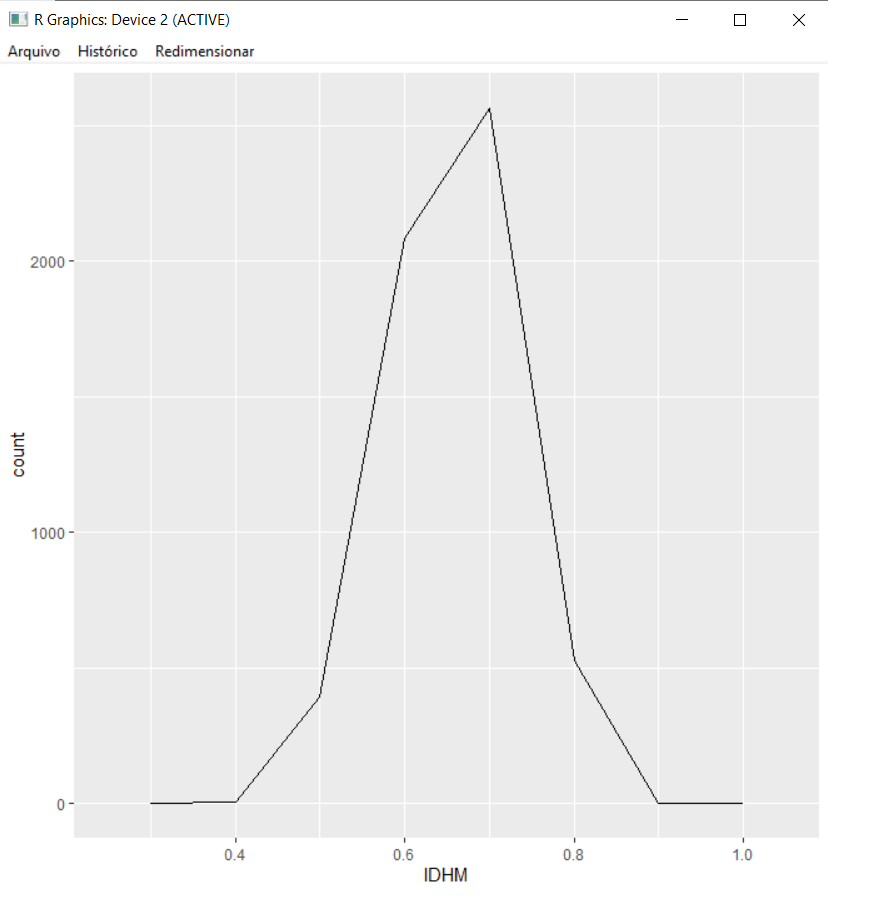
\includegraphics[scale=0.6]{chapter-03-case-02-img-01}
  \legend{Fonte: O autor}
\end{figure}

Já na figura, é mostrado a distribuição da população estrangeira sobre a população total de uma cidade.

...




